% ---------------------------------------------------------------
% 3.2  V-MARCH Overview
% ---------------------------------------------------------------
\subsection{\ours Overview}
\label{sec:overview}

\begin{figure*}[t]
    \centering
    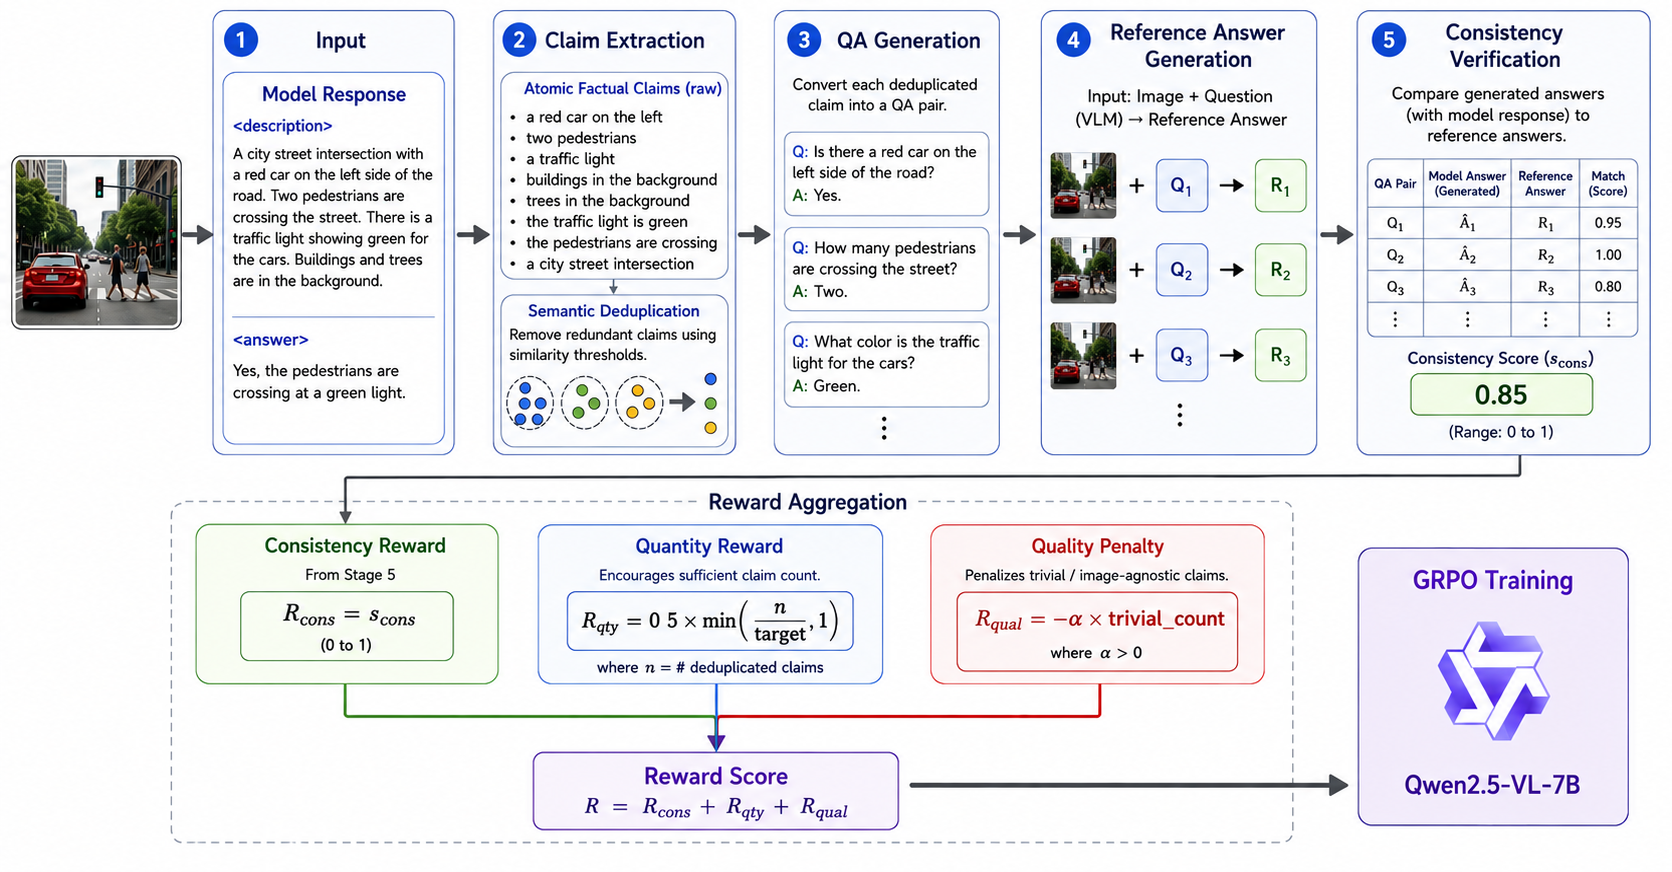
\includegraphics[width=\textwidth]{figures/pipeline.png}
    \caption{Overview of the \ours pipeline. Given a model-generated response,
    \ours first extracts atomic factual claims from the generated description
    and removes semantically redundant claims. Each remaining claim is converted
    into a visual question-answer pair, where the answer is implied by the
    generated description. The VLM then answers the same questions using the
    original image, producing image-grounded reference answers. The consistency
    between the implied answers and the reference answers is verified through
    majority voting. In addition, Visual Evidence Calibration (VEC) calibrates
    the reward by encouraging diverse claims, rewarding sufficient claim
    coverage, and penalizing claims answerable from degraded visual evidence.}
    \label{fig:pipeline}
\end{figure*}

\ours adapts the information-asymmetric Proposer--Checker paradigm of
MARCH~\cite{li2026march} to the visual domain and extends it with a
fourth specialized agent, the \textbf{Calibrator}, designed to address
failure modes unique to visual self-verification.
As illustrated in Figure~\ref{fig:pipeline}, \ours orchestrates four
agents in a sequential pipeline:

\begin{itemize}[leftmargin=1.5em,itemsep=2pt]
  \item \textbf{Solver.} Generates a structured response
        $y=(y^{\mathrm{desc}}, y^{\mathrm{ans}})$ conditioned on the
        image--instruction pair $(I, q)$, where $y^{\mathrm{desc}}$
        is a free-form visual description and $y^{\mathrm{ans}}$ is
        the task answer.

  \item \textbf{Proposer.} Decomposes $y^{\mathrm{desc}}$ into
        deduplicated atomic factual claims and converts each claim into
        a visual question-answer pair, yielding the claim set
        $\mathcal{Q} = \{(v_i, a_i)\}_{i=1}^{n}$.

  \item \textbf{Checker.} Answers each question $v_i$ using only the
        original image $I$, producing image-grounded reference answers
        $\{a_i'\}$ and verifying consistency with $\{a_i\}$ via
        majority voting. This \emph{information asymmetry}---the
        Checker sees the image but not $y^{\mathrm{desc}}$---breaks
        the self-confirmation bias of single-model verification.

  \item \textbf{Calibrator.} Audits the reliability of the
        verification signal by (i) penalizing redundant or
        image-agnostic claims that inflate the reward without genuine
        visual grounding, and (ii) rewarding sufficient claim
        coverage. The Calibrator is our primary contribution over the
        original MARCH framework and is described in detail in
        Section~\ref{sec:calibrator}.
\end{itemize}

The final self-verifying reward aggregates signals from the Checker and
the Calibrator:
\begin{equation}
    R_{\mathrm{SV}}(I,q,y)
    = \underbrace{R_{\mathrm{cons}}}_{\text{Checker}}
    + \underbrace{R_{\mathrm{cnt}} + R_{\mathrm{qual}}}_{\text{Calibrator}}.
    \label{eq:reward_total}
\end{equation}
This reward is used directly as the GRPO training signal,
requiring no human annotation or external supervision.


% ---------------------------------------------------------------
% 3.3  Proposer and Checker: Claim-Level Self-Verification
% ---------------------------------------------------------------
\subsection{Proposer and Checker: Claim-Level Self-Verification}
\label{sec:claim_level_verification}

\paragraph{Proposer: Claim Extraction and Deduplication.}
Given $y^{\mathrm{desc}}$, the Proposer first extracts atomic factual
claims:
\begin{equation}
    \mathcal{C} = \{c_1,\ldots,c_m\} = \mathrm{Extract}(y^{\mathrm{desc}}),
\end{equation}
where each $c_i$ is a short, self-contained statement about a single
visual fact (object existence, color, quantity, or spatial relation).
To prevent reward hacking via repetition, semantically overlapping
claims are removed using cosine similarity over sentence embeddings
$\phi(\cdot)$:
\begin{equation}
    \mathrm{sim}(c_i,c_j)
    = \frac{\phi(c_i)^\top \phi(c_j)}{\|\phi(c_i)\|\cdot\|\phi(c_j)\|}.
\end{equation}
Pairs exceeding a type-aware threshold are merged, yielding the
deduplicated set $\mathcal{C}^{\ast}=\{c_1^{\ast},\ldots,c_n^{\ast}\}$,
$n \leq m$.
Each $c_i^{\ast}$ is then converted into a visual QA pair
$(v_i, a_i) = \mathrm{QA}(c_i^{\ast})$, where $a_i$ is the answer
implied by the claim.

\paragraph{Checker: Image-Grounded Verification.}
The Checker receives only the image $I$ and each question $v_i$,
with no access to $y^{\mathrm{desc}}$. It generates a reference answer
\begin{equation}
    a_i' = \mathrm{Ans}(I, v_i),
\end{equation}
and verifies consistency with the claim-implied answer via majority
voting over $K$ independent runs:
\begin{equation}
    z_i = \mathbbm{1}\!\left[\sum_{k=1}^{K} z_i^{(k)} > \tfrac{K}{2}\right],
    \qquad z_i^{(k)} = f_{\mathrm{ver}}(a_i, a_i').
\end{equation}
The resulting consistency reward is
\begin{equation}
    R_{\mathrm{cons}} = \frac{1}{n}\sum_{i=1}^{n} z_i,
\end{equation}
measuring the fraction of claims that are supported by
image-grounded evidence.


% ---------------------------------------------------------------
% 3.4  Calibrator: Visual Evidence Calibration
% ---------------------------------------------------------------
\subsection{Calibrator: Visual Evidence Calibration}
\label{sec:calibrator}

The Checker's consistency reward $R_{\mathrm{cons}}$ alone is
susceptible to three degenerate behaviors specific to visual
self-verification: (1)~a model can repeat near-identical claims to
inflate the score; (2)~it can produce very few but easily-verified
claims to obtain a stable reward while remaining under-informative;
(3)~it can generate generic claims (e.g., \textit{``there are objects
in the image''}) whose answers follow from language priors rather than
genuine visual perception.
We introduce the \textbf{Calibrator} agent to counteract all three
failure modes through two complementary reward components.

\paragraph{Informativeness Reward.}
To encourage responses that cover the image sufficiently, the
Calibrator adds a claim-count reward proportional to the number of
deduplicated claims $n$, capped at a target $n_{\mathrm{target}}$:
\begin{equation}
    R_{\mathrm{cnt}}
    = \lambda_{\mathrm{cnt}}
      \cdot \min\!\left(\tfrac{n}{n_{\mathrm{target}}},\, 1\right),
\end{equation}
with $\lambda_{\mathrm{cnt}}=0.5$ so that factual consistency remains
the dominant signal.
Note that semantic deduplication (Section~\ref{sec:claim_level_verification})
already prevents redundant claims from contributing to $n$, jointly
addressing failure mode~(1) and~(2).

\paragraph{Visual-Dependence Penalty.}
To detect image-agnostic claims (failure mode~3), the Calibrator
constructs a degraded image $\tilde{I}$ by applying heavy Gaussian
blur, grayscale conversion, and horizontal flipping to $I$.
It then re-answers each question with the degraded image:
\begin{equation}
    \tilde{a}_i = \mathrm{Ans}(\tilde{I},\, v_i).
\end{equation}
If $\tilde{a}_i$ remains consistent with the original reference answer
$a_i'$, the claim is marked as trivial---i.e., answerable without
meaningful visual content:
\begin{equation}
    t_i = \mathbbm{1}\!\left[
        f_{\mathrm{ver}}(\tilde{a}_i, a_i') = 1
        % \;\land\;
        % a_i' \neq \texttt{unknown}
        % \;\land\;
        % \tilde{a}_i \neq \texttt{unknown}
    \right].
\end{equation}
The Calibrator penalizes trivial claims proportionally:
\begin{equation}
    R_{\mathrm{qual}} = -\lambda_{\mathrm{qual}} \sum_{i=1}^{n} t_i,
\end{equation}
pushing the model toward claims that require genuine image grounding.

\paragraph{Final Reward.}
Combining the Checker and Calibrator signals, the total reward
used for GRPO training is (cf.\ Eq.~\eqref{eq:reward_total}):
\begin{equation}
    R_{\mathrm{SV}}(I,q,y)
    = R_{\mathrm{cons}} + R_{\mathrm{cnt}} + R_{\mathrm{qual}}.
\end{equation}
The three terms are complementary: $R_{\mathrm{cons}}$ enforces
factual grounding; $R_{\mathrm{cnt}}$ promotes visual coverage; and
$R_{\mathrm{qual}}$ filters out image-agnostic claims.
Together, the four-agent pipeline provides a reliable,
annotation-free reward signal for scalable hallucination mitigation.
